\documentclass[11pt,a4paper]{article}

% ---- Packages ----------------------------------------------------------
\usepackage[utf8]{inputenc}
\usepackage[T1]{fontenc}
\usepackage{lmodern}
\usepackage[margin=0.85in]{geometry}
\usepackage{microtype}
\usepackage{amsmath}
\usepackage{amssymb}
\usepackage{titlesec}
\usepackage{enumitem}
\usepackage{booktabs}
\usepackage{array}
\usepackage{tabularx}
\usepackage{xcolor}
\usepackage{graphicx}
\usepackage{fancyhdr}
\usepackage{tikz}
\usetikzlibrary{positioning, arrows.meta, shapes.geometric, fit, calc, backgrounds, decorations.pathreplacing, shadows.blur}
\usepackage[hidelinks,colorlinks=true,linkcolor=black,citecolor=violet,urlcolor=violet]{hyperref}
\usepackage{parskip}
\usepackage{float}
\usepackage{tcolorbox}
\tcbuselibrary{skins, breakable}

% ---- Colour palette ----------------------------------------------------
\definecolor{primary}{HTML}{4338CA}
\definecolor{primarylight}{HTML}{E0E7FF}
\definecolor{secondary}{HTML}{0E7490}
\definecolor{secondarylight}{HTML}{CFFAFE}
\definecolor{accent}{HTML}{C2410C}
\definecolor{accentlight}{HTML}{FFEDD5}
\definecolor{ink}{HTML}{1E1B4B}
\definecolor{mute}{HTML}{64748B}
\definecolor{mutelight}{HTML}{F1F5F9}
\definecolor{ok}{HTML}{15803D}
\definecolor{warn}{HTML}{B91C1C}
\definecolor{precfp}{HTML}{0F766E}
\definecolor{precfplight}{HTML}{CCFBF1}
\definecolor{precint}{HTML}{7C3AED}
\definecolor{precintlight}{HTML}{EDE9FE}
\definecolor{clsA}{HTML}{0F766E}
\definecolor{clsAlight}{HTML}{CCFBF1}
\definecolor{clsB}{HTML}{B45309}
\definecolor{clsBlight}{HTML}{FEF3C7}
\definecolor{clsC}{HTML}{BE185D}
\definecolor{clsClight}{HTML}{FCE7F3}
\definecolor{clsN}{HTML}{4338CA}
\definecolor{clsNlight}{HTML}{E0E7FF}

% ---- TikZ styles -------------------------------------------------------
\tikzset{
  block/.style    = {rectangle, rounded corners=4pt, draw=primary, thick,
                     fill=primarylight, minimum width=2.4cm, minimum height=0.85cm,
                     align=center, font=\small},
  brain/.style    = {rectangle, rounded corners=4pt, draw=secondary, very thick,
                     fill=secondarylight, minimum width=2.6cm, minimum height=1.0cm,
                     align=center, font=\small},
  art/.style      = {rectangle, rounded corners=4pt, draw=accent, thick,
                     fill=accentlight, minimum width=2.4cm, minimum height=0.85cm,
                     align=center, font=\small},
  hub/.style      = {rectangle, rounded corners=4pt, draw=primary, very thick,
                     fill=primarylight, minimum width=4.2cm, minimum height=2.4cm,
                     align=left, font=\small},
  iot/.style      = {rectangle, rounded corners=3pt, draw=mute, thick,
                     fill=mutelight, minimum width=1.9cm, minimum height=0.7cm,
                     align=center, font=\scriptsize},
  data/.style     = {rectangle, rounded corners=3pt, draw=mute, thick,
                     fill=mutelight, minimum width=2.2cm, minimum height=0.8cm,
                     align=center, font=\small},
  decision/.style = {diamond, draw=accent, thick, fill=accentlight, aspect=1.5,
                     inner sep=1pt, align=center, font=\small},
  signal/.style   = {rectangle, rounded corners=3pt, draw=warn, thick,
                     fill=red!8, minimum width=2.2cm, minimum height=0.8cm,
                     align=center, font=\small},
  pkt/.style      = {rectangle, draw=secondary!70, thick, fill=secondarylight,
                     minimum width=0.5cm, minimum height=0.5cm,
                     inner sep=1pt, font=\tiny},
  bead/.style     = {circle, draw=primary!70, thick, fill=primarylight,
                     inner sep=1pt, minimum size=0.45cm, font=\tiny},
  result/.style   = {rectangle, rounded corners=3pt, draw=accent, thick,
                     fill=accentlight, minimum width=2.4cm, minimum height=0.8cm,
                     align=center, font=\small},
  int8/.style     = {rectangle, rounded corners=3pt, draw=precint, thick,
                     fill=precintlight, minimum width=3.2cm, minimum height=0.7cm,
                     align=center, font=\small},
  fp16/.style     = {rectangle, rounded corners=3pt, draw=precfp, very thick,
                     fill=precfplight, minimum width=3.2cm, minimum height=1.3cm,
                     align=center, font=\small},
  ar/.style       = {-{Latex[length=2mm,width=1.6mm]}, thick, draw=ink!75},
  dar/.style      = {-{Latex[length=2mm,width=1.6mm]}, thick, draw=ink!75, dashed},
}

% ---- tcolorbox styles --------------------------------------------------
\tcbset{
  snap/.style={colback=primarylight, colframe=primary, boxrule=0.6pt,
               arc=2pt, left=8pt, right=8pt, top=6pt, bottom=6pt,
               fonttitle=\bfseries, coltitle=white, colbacktitle=primary,
               title={\strut SNAPSHOT}},
  idea/.style={colback=secondarylight, colframe=secondary!60, boxrule=0.5pt,
               arc=2pt, left=8pt, right=8pt, top=5pt, bottom=5pt,
               fonttitle=\bfseries\small, coltitle=white, colbacktitle=secondary,
               title={\strut KEY IDEA}},
  warnbox/.style={colback=accentlight, colframe=accent!60, boxrule=0.5pt,
                  arc=2pt, left=8pt, right=8pt, top=5pt, bottom=5pt,
                  fonttitle=\bfseries\small, coltitle=white, colbacktitle=accent,
                  title={\strut WATCH OUT}},
}

% ---- Header / Footer ---------------------------------------------------
\pagestyle{fancy}
\fancyhf{}
\fancyhead[L]{\small\color{primary}\textbf{IoT Gateway Anomaly Detection}}
\fancyhead[R]{\small\color{mute}Madhav Dogra}
\fancyfoot[C]{\small\color{mute}\thepage}
\renewcommand{\headrulewidth}{0pt}

% ---- Section format ----------------------------------------------------
\titleformat{\section}
  {\normalfont\LARGE\bfseries\color{primary}}
  {\textcolor{accent}{\thesection}\hspace{0.4em}}{0pt}{}
\titlespacing*{\section}{0pt}{14pt}{6pt}

\titleformat{\subsection}
  {\normalfont\large\bfseries\color{ink}}
  {\textcolor{secondary}{\thesubsection}\hspace{0.3em}}{0pt}{}
\titlespacing*{\subsection}{0pt}{8pt}{2pt}

\setlength{\parskip}{4pt}

% =======================================================================
\begin{document}

% ---- Title block ------------------------------------------------------
\begin{center}
{\color{primary}\rule{\linewidth}{1pt}}\\[6pt]
{\Huge\bfseries\color{ink} Flow-Pattern Anomaly Detection at the IoT Gateway} \\[6pt]
{\Large\color{secondary} A pre-trained Mamba detector for known and zero-day attacks on smart-home devices} \\[4pt]
{\color{mute}\rule{0.6\linewidth}{0.3pt}}\\[4pt]
{\normalsize\color{mute} Madhav Dogra \quad\textbullet\quad Final Project Proposal}
\end{center}

\vspace{4pt}

\begin{tcolorbox}[snap]
A detector that sits at the home gateway and inspects every flow to or from a smart-home device. \textbf{Known attacks} are caught by a supervised classifier; \textbf{zero-day attacks} by a one-class anomaly scorer. Both heads ride a single \textbf{Mamba} encoder pre-trained on benign traffic. The detector runs in two operating modes --- a low-power \textbf{default} that runs continuously, and an admin-switched \textbf{strong} mode with the full pipeline and SHAP attributions. New attack types are absorbed by re-training only the lightweight classifier head, not the encoder. Target: $<$10\,ms p95 per flow on Raspberry-Pi-class hardware after int8 quantisation.
\end{tcolorbox}

% =======================================================================
\section{The setting}

The target environment is the modern smart home. The device population includes \textbf{IP cameras, motion and environmental sensors, smart bulbs, voice assistants, thermostats, video doorbells, smart plugs, and the gateway itself}. CICIoT2023, the primary training dataset, is dominated by exactly this device class: 105 real consumer IoT devices, 33 attack types, 7 attack categories.

\subsection{Why these devices are the soft layer}
They ship with default credentials, run firmware that is rarely updated, lack the compute to host any endpoint security agent, and are often physically accessible. The Mirai botnet --- built almost entirely from compromised IP cameras and home routers --- is the canonical demonstration that this surface is exploitable at scale. In a defence context the stakes rise: field sensors, surveillance equipment and base infrastructure are high-value, low-trust devices that cannot be hardened one by one.

\subsection{Why the gateway is the right vantage point}
Putting software \emph{on} the devices is not possible. Watching them on the network is. The gateway is the single point through which every device flow passes on its way upstream, and the only place where modern compute can sit without instrumenting the device fleet. The trade-off: gateway hardware is small (Raspberry-Pi-class, single-digit watts), so the detector must be lightweight. This one constraint shapes every architectural decision that follows.

% ---- Figure 1: topology -----------------------------------------------
\begin{figure}[H]
\centering
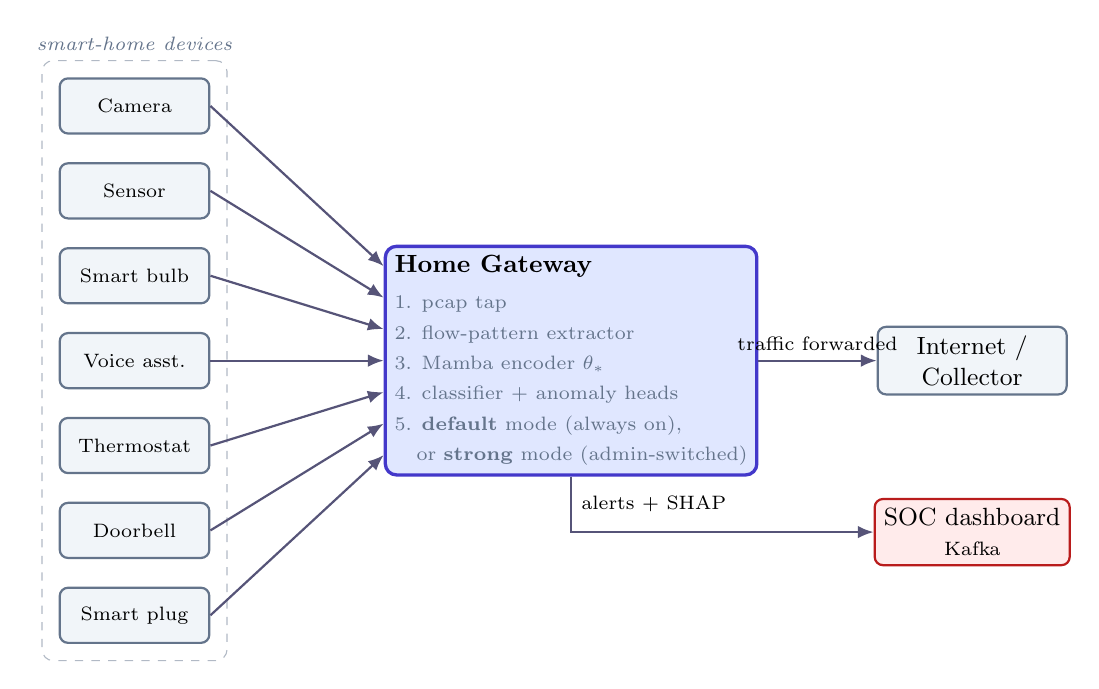
\begin{tikzpicture}[node distance=0.35cm and 1.2cm]

  \node[iot] (cam)   {Camera};
  \node[iot, below=of cam]   (sen) {Sensor};
  \node[iot, below=of sen]   (bulb){Smart bulb};
  \node[iot, below=of bulb]  (va)  {Voice asst.};
  \node[iot, below=of va]    (thr) {Thermostat};
  \node[iot, below=of thr]   (door){Doorbell};
  \node[iot, below=of door]  (plug){Smart plug};

  \node[draw=mute!50, dashed, rounded corners, fit=(cam)(plug), inner sep=6pt,
        label={[font=\scriptsize\itshape, mute]above:smart-home devices}] (grp) {};

  \node[hub, right=2.2cm of va] (gw)
       {\textbf{Home Gateway} \\[2pt]
        \scriptsize \color{mute} 1. pcap tap \\
        \scriptsize \color{mute} 2. flow-pattern extractor \\
        \scriptsize \color{mute} 3. Mamba encoder $\theta_*$ \\
        \scriptsize \color{mute} 4. classifier + anomaly heads \\
        \scriptsize \color{mute} 5. \textbf{default} mode (always on), \\
        \scriptsize \color{mute} \quad or \textbf{strong} mode (admin-switched)};

  \node[data, right=1.5cm of gw, minimum width=2.4cm] (cc)
       {Internet / \\ Collector};
  \node[signal, below=1.3cm of cc, minimum width=2.4cm] (soc) {SOC dashboard \\ \scriptsize Kafka};

  \draw[ar] (cam.east)  -- ([yshift=1.2cm]gw.west);
  \draw[ar] (sen.east)  -- ([yshift=0.8cm]gw.west);
  \draw[ar] (bulb.east) -- ([yshift=0.4cm]gw.west);
  \draw[ar] (va.east)   -- (gw.west);
  \draw[ar] (thr.east)  -- ([yshift=-0.4cm]gw.west);
  \draw[ar] (door.east) -- ([yshift=-0.8cm]gw.west);
  \draw[ar] (plug.east) -- ([yshift=-1.2cm]gw.west);

  \draw[ar] (gw.east) -- node[above, font=\scriptsize]{traffic forwarded} (cc.west);
  \draw[ar] (gw.south) |- node[pos=0.25, right, font=\scriptsize]{alerts + SHAP} (soc.west);

\end{tikzpicture}
\caption*{\small\textit{Figure 1 --- The detector lives inside the home gateway. Device traffic continues upstream unchanged; alerts and SHAP attributions are sent out-of-band to a SOC dashboard.}}
\end{figure}

% =======================================================================
\section{What the detector must do}

Four properties, in priority order, plus one hard constraint.

\begin{enumerate}[leftmargin=*, itemsep=3pt]
  \item \textbf{Catch known attacks} with high precision --- DDoS, reconnaissance, brute force, Mirai-style botnet traffic. The supervised classifier owns this.
  \item \textbf{Catch unknown (zero-day) attacks.} A detector that only recognises known patterns misses the next new thing. The one-class anomaly scorer owns this: it learns ``normal'' and flags whatever does not fit, without ever training on the attack.
  \item \textbf{Work on encrypted traffic.} Payloads are opaque, so the detector reads flow metadata only --- packet sizes, directions, timings, flag distributions, header fields.
  \item \textbf{Explain every alert.} ``The model said so'' is not actionable. Every flagged flow carries an attribution of which features drove the decision, so an analyst can act on it.
\end{enumerate}

\textbf{The constraint:} all of this runs at the gateway, on small hardware, in under 10\,ms per flow. Existing approaches each cover one or two of these. Signature firewalls catch known attacks but miss zero-days. Enterprise IDS is tuned for human traffic and false-alarms on periodic machine-to-machine patterns. Transformer detectors are accurate but do not fit on edge hardware. Most academic work benchmarks on a single dataset and never measures evasion. The gap is a detector that does all four \emph{and} is stress-tested.

% =======================================================================
\section{The input representation}

Conventional IoT IDS collapses each flow into a vector of $\sim$80 summary statistics (mean packet size, IAT standard deviation, flag counts, $\ldots$) before the model sees it. This is convenient but \emph{permutation-invariant} --- shuffle the packets and the statistics do not change --- which destroys the temporal structure that attack signatures live in.

\begin{tcolorbox}[idea]
\textbf{Keep the order.} A flow is the first $K\!\approx\!32$ packets of the connection, kept as an ordered sequence $\mathbf{x} = (p_1, \ldots, p_K)$. Each $p_t$ is a small per-packet feature vector --- size, direction, inter-arrival time, TCP flags, header fields. A sequence model can then learn what a normal sequence looks like, and what a malicious one looks like.
\end{tcolorbox}

% ---- Figure 2: representation contrast --------------------------------
\begin{figure}[H]
\centering
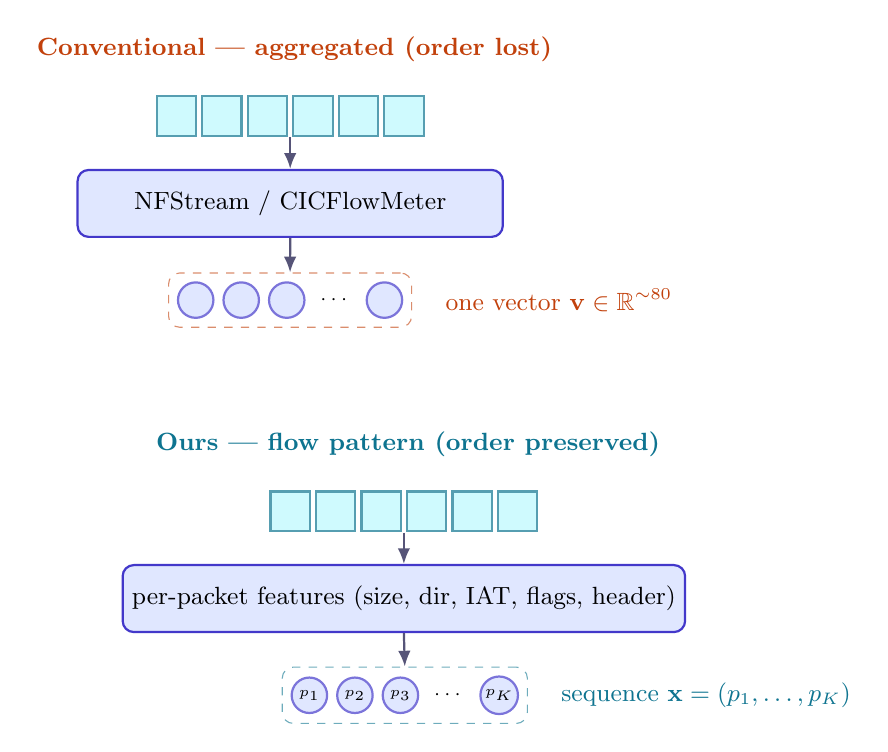
\begin{tikzpicture}[node distance=0.4cm and 0.9cm]

  \node[font=\bfseries\small, color=accent] (lhd) {Conventional --- aggregated (order lost)};

  \node[pkt, below=0.3cm of lhd, xshift=-1.5cm] (lp1) {};
  \node[pkt, right=0.05cm of lp1] (lp2) {};
  \node[pkt, right=0.05cm of lp2] (lp3) {};
  \node[pkt, right=0.05cm of lp3] (lp4) {};
  \node[pkt, right=0.05cm of lp4] (lp5) {};
  \node[pkt, right=0.05cm of lp5] (lp6) {};
  \node[fit=(lp1)(lp6), inner sep=0pt] (lpkts) {};

  \node[block, below=0.4cm of lpkts, minimum width=5.4cm] (lagg)
       {\small NFStream / CICFlowMeter};

  \node[bead, below=0.55cm of lagg, xshift=-1.2cm] (lf1) {};
  \node[bead, right=0.1cm of lf1] (lf2) {};
  \node[bead, right=0.1cm of lf2] (lf3) {};
  \node[right=0.06cm of lf3, font=\scriptsize] (ldots) {$\cdots$};
  \node[bead, right=0.06cm of ldots] (lf4) {};
  \node[draw=accent!60, dashed, rounded corners, fit=(lf1)(lf4), inner sep=3pt] (lvec) {};
  \node[right=0.3cm of lvec, font=\small, color=accent] {one vector $\mathbf{v}\in\mathbb{R}^{\sim 80}$};

  \draw[ar] (lpkts.south) -- (lagg.north);
  \draw[ar] (lagg.south) -- (lvec.north);

  \node[font=\bfseries\small, color=secondary, below=1.2cm of lvec, xshift=1.5cm] (rhd)
       {Ours --- flow pattern (order preserved)};

  \node[pkt, below=0.3cm of rhd, xshift=-1.5cm] (rp1) {};
  \node[pkt, right=0.05cm of rp1] (rp2) {};
  \node[pkt, right=0.05cm of rp2] (rp3) {};
  \node[pkt, right=0.05cm of rp3] (rp4) {};
  \node[pkt, right=0.05cm of rp4] (rp5) {};
  \node[pkt, right=0.05cm of rp5] (rp6) {};
  \node[fit=(rp1)(rp6), inner sep=0pt] (rpkts) {};

  \node[block, below=0.4cm of rpkts, minimum width=5.4cm] (ragg)
       {\small per-packet features (size, dir, IAT, flags, header)};

  \node[bead, below=0.55cm of ragg, xshift=-1.2cm] (rf1) {$p_1$};
  \node[bead, right=0.1cm of rf1] (rf2) {$p_2$};
  \node[bead, right=0.1cm of rf2] (rf3) {$p_3$};
  \node[right=0.06cm of rf3, font=\scriptsize] (rdots) {$\cdots$};
  \node[bead, right=0.06cm of rdots] (rf4) {$p_K$};
  \node[draw=secondary!60, dashed, rounded corners, fit=(rf1)(rf4), inner sep=3pt] (rvec) {};
  \node[right=0.3cm of rvec, font=\small, color=secondary] {sequence $\mathbf{x}=(p_1,\ldots,p_K)$};

  \draw[ar] (rpkts.south) -- (ragg.north);
  \draw[ar] (ragg.south) -- (rvec.north);

\end{tikzpicture}
\caption*{\small\textit{Figure 2 --- Two ways to feed a flow to a model. Aggregation collapses everything into one vector and drops ordering; the flow-pattern keeps the packets in order so a sequence model can use the temporal structure.}}
\end{figure}

\subsection{Preprocessing --- transforms before the model}
Traffic features are heavy-tailed: a handful of flows carry megabytes while most carry a few hundred bytes; a few connections idle for seconds while most are sub-millisecond. Raw, this long right tail dominates every distance computation and swamps clustering and one-class scoring.

\begin{tcolorbox}[idea]
Apply $\log(1+x)$ to the heavy-tailed per-packet and per-flow features. It compresses the tail, makes each distribution near-symmetric, and tightens the class clusters. Standardise (zero-mean, unit-variance) \emph{after} the log. The \textbf{Yeo--Johnson} power transform generalises this --- it learns the best exponent per feature and handles zeros and negatives automatically (one \texttt{scikit-learn} call); $\log(1+x)$ is the transparent fallback.
\end{tcolorbox}

\begin{tcolorbox}[warnbox]
$\log$ and $\exp$ move data in \emph{opposite} directions. For positive, right-skewed traffic features, $\log$ compresses large values toward the bulk (good); $e^{x}$ expands them and stretches the tail further (worse). The compacting transform here is the logarithm, not the exponential.
\end{tcolorbox}

% ---- Figure 3: distribution compaction --------------------------------
\begin{figure}[H]
\centering
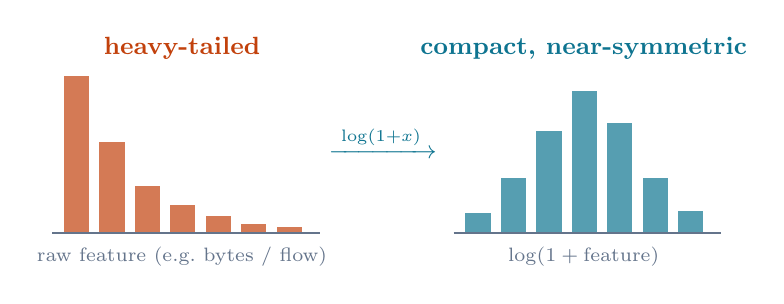
\begin{tikzpicture}

  \begin{scope}
    \foreach \x/\h in {0/2.0, 0.45/1.15, 0.9/0.6, 1.35/0.35, 1.8/0.22, 2.25/0.12, 2.7/0.07}
       {\fill[accent!70] (\x,0) rectangle ++(0.32,\h);}
    \draw[mute, thick] (-0.15,0) -- (3.25,0);
    \node[font=\scriptsize\color{mute}] at (1.5,-0.3) {raw feature (e.g.\ bytes / flow)};
    \node[font=\bfseries\small\color{accent}] at (1.5, 2.35) {heavy-tailed};
  \end{scope}

  \node[font=\small\color{secondary}] at (4.05, 1.15) {$\xrightarrow{\;\log(1+x)\;}$};

  \begin{scope}[shift={(5.1,0)}]
    \foreach \x/\h in {0/0.25, 0.45/0.7, 0.9/1.3, 1.35/1.8, 1.8/1.4, 2.25/0.7, 2.7/0.28}
       {\fill[secondary!70] (\x,0) rectangle ++(0.32,\h);}
    \draw[mute, thick] (-0.15,0) -- (3.25,0);
    \node[font=\scriptsize\color{mute}] at (1.5,-0.3) {$\log(1+\text{feature})$};
    \node[font=\bfseries\small\color{secondary}] at (1.5, 2.35) {compact, near-symmetric};
  \end{scope}

\end{tikzpicture}
\caption*{\small\textit{Figure 3 --- The log transform on a heavy-tailed traffic feature. The long right tail (amber) is pulled into a compact, roughly symmetric distribution (teal), so distances and one-class scores reflect the bulk of the data rather than a few outliers.}}
\end{figure}

% =======================================================================
\section{Feature significance and visualisation}

Two questions get conflated and should be kept apart: \emph{which input dimensions carry class signal}, and \emph{do the classes separate in the chosen representation}. They need different tools.

\begin{tcolorbox}[idea]
Rank features with \textbf{mutual information} and \textbf{SHAP}. Use \textbf{t-SNE / UMAP only to confirm} separability. t-SNE and UMAP are visualisation tools, not feature rankers: their two output axes are nonlinear blends of \emph{all} the inputs, with no per-feature loadings to read off. Reading a feature ranking off a t-SNE plot is the mistake to avoid.
\end{tcolorbox}

Mutual information is the univariate, model-free relevance score and is the feature-selection step in the pipeline; it cuts dimensionality by more than half with negligible accuracy loss. SHAP, already used for per-alert explanation, doubles as a global importance ranking by averaging $|$attribution$|$ across flows. Permutation importance is a cheap cross-check. t-SNE/UMAP then answer one question only: do benign traffic and each attack category fall into distinct clusters. Two cautions: cluster \emph{sizes} and the \emph{distances between} clusters in a t-SNE plot are not meaningful (only local neighbourhoods are preserved), and the picture changes with perplexity. It is a qualitative diagnostic, never a measurement.

Hand-selecting input dimensions applies to the classical baselines (XGBoost / Isolation Forest on the aggregated statistics). The Mamba arm consumes the ordered sequence and learns its own representation $\mathbf{z}$; for that arm the high-value use of t-SNE/UMAP is to visualise $\mathbf{z}$ coloured by class, confirming the encoder built a separable space --- the precondition the anomaly head depends on.

% ---- Figure 4: rank then visualise ------------------------------------
\begin{figure}[H]
\centering
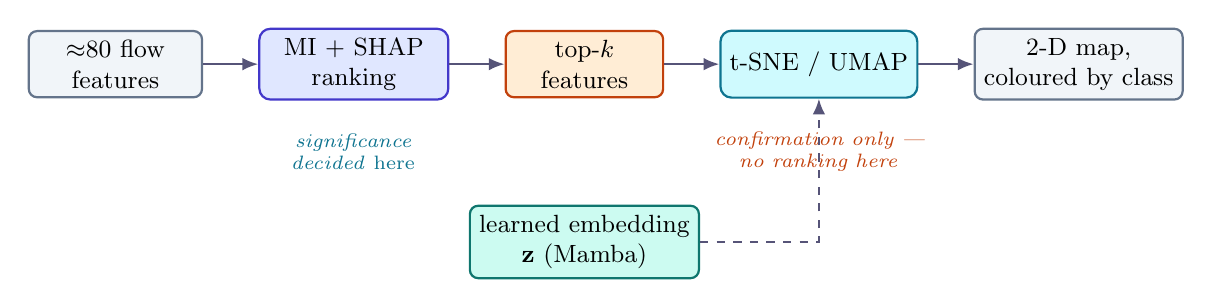
\begin{tikzpicture}[node distance=0.55cm and 0.7cm]

  \node[data, minimum width=2.2cm] (feats) {$\approx$80 flow \\ features};
  \node[block, right=of feats, fill=primarylight, draw=primary] (rank) {MI $+$ SHAP \\ ranking};
  \node[result, right=of rank, minimum width=2.0cm] (topk) {top-$k$ \\ features};
  \node[block, right=of topk, fill=secondarylight, draw=secondary] (tsne) {t-SNE / UMAP};
  \node[data, right=of tsne, minimum width=2.4cm] (map) {2-D map, \\ coloured by class};

  \draw[ar] (feats) -- (rank);
  \draw[ar] (rank) -- (topk);
  \draw[ar] (topk) -- (tsne);
  \draw[ar] (tsne) -- (map);

  \node[font=\scriptsize\itshape\color{secondary}, below=0.3cm of rank, align=center, text width=2.6cm]
       {significance decided \emph{here}};
  \node[font=\scriptsize\itshape\color{accent}, below=0.3cm of tsne, align=center, text width=2.6cm]
       {confirmation only --- \\ no ranking here};

  \node[result, below=1.35cm of topk, fill=precfplight, draw=precfp, minimum width=2.6cm] (z)
       {learned embedding \\ $\mathbf{z}$ (Mamba)};
  \draw[dar] (z.east) -| (tsne.south);

\end{tikzpicture}
\caption*{\small\textit{Figure 4 --- Rank, then visualise. Feature significance is produced by mutual information and SHAP (indigo); t-SNE/UMAP (teal) only confirms that the kept features separate the classes. For the Mamba arm the same plot is applied to the learned embedding $\mathbf{z}$ (dashed branch).}}
\end{figure}

% =======================================================================
\section{The architecture}

A single \textbf{Mamba encoder} processes the sequence $\mathbf{x}$ and produces a fixed-size embedding $\mathbf{z}$. Two heads read $\mathbf{z}$ in parallel:

\begin{itemize}[leftmargin=*, itemsep=2pt]
  \item \textbf{Classifier head} --- a small MLP $\to$ softmax over the 7 known attack categories from CICIoT2023. Trained with focal loss to handle the heavy class imbalance.
  \item \textbf{Anomaly head} --- a one-class deep SVDD scorer trained \emph{only on benign embeddings}. It does not know about any specific attack; it measures distance from ``normal.''
\end{itemize}

\begin{tcolorbox}[idea]
\textbf{The anomaly head reads a \emph{projected} embedding} $\mathbf{z}_\text{ano} = g_\phi(\mathbf{z})$ from a small learnable MLP ($\mathbb{R}^{128} \to \mathbb{R}^{32}$). One-class scorers suffer the curse of dimensionality: in high dimensions, distances concentrate and lose discriminative power. Projecting to a smaller anomaly space sharpens the score. The projection is trained jointly with the SVDD objective.
\end{tcolorbox}

% ---- Figure 5: architecture -------------------------------------------
\begin{figure}[H]
\centering
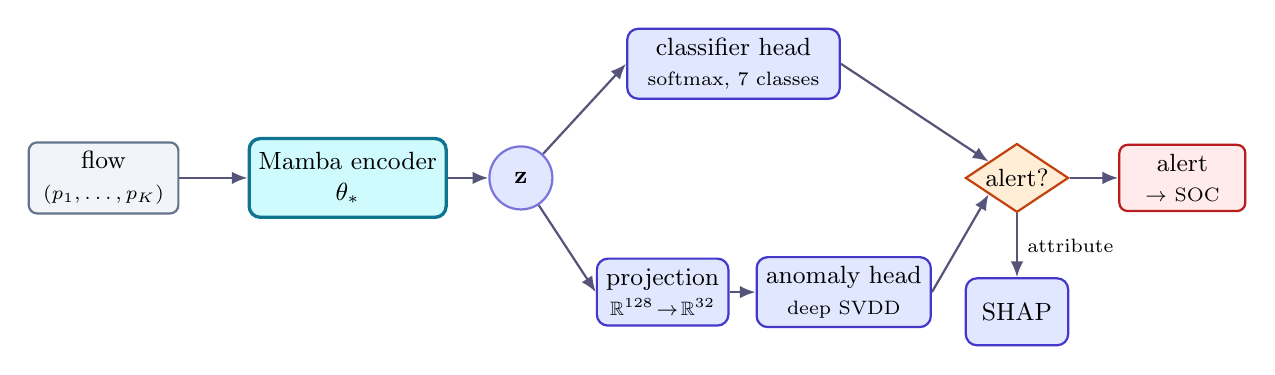
\begin{tikzpicture}

  \node[data, minimum width=1.9cm] (flow) at (0,0) {flow \\ \scriptsize $(p_1,\dots,p_K)$};
  \node[brain, minimum width=2.4cm] (enc) at (3.1,0) {Mamba encoder \\ $\theta_*$};
  \node[bead, minimum size=0.8cm, font=\small] (z) at (5.3,0) {$\mathbf{z}$};

  \node[block, minimum width=2.7cm] (cls) at (8.0,1.45)
       {classifier head \\ \scriptsize softmax, 7 classes};
  \node[block, minimum width=1.5cm] (proj) at (7.1,-1.45)
       {projection \\ \scriptsize $\mathbb{R}^{128}\!\to\!\mathbb{R}^{32}$};
  \node[block, minimum width=1.8cm] (ano) at (9.4,-1.45)
       {anomaly head \\ \scriptsize deep SVDD};

  \node[decision] (fuse) at (11.6,0) {alert?};
  \node[signal, minimum width=1.6cm] (out) at (13.7,0) {alert \\ \scriptsize $\to$ SOC};
  \node[block, minimum width=1.3cm] (shap) at (11.6,-1.7) {SHAP};

  \draw[ar] (flow) -- (enc);
  \draw[ar] (enc) -- (z);
  \draw[ar] (z) -- (cls.west);
  \draw[ar] (z) -- (proj.west);
  \draw[ar] (proj) -- (ano);
  \draw[ar] (cls.east) -- (fuse.150);
  \draw[ar] (ano.east) -- (fuse.210);
  \draw[ar] (fuse.east) -- (out.west);
  \draw[ar] (fuse.270) -- node[right, font=\scriptsize]{attribute} (shap.north);

\end{tikzpicture}
\caption*{\small\textit{Figure 5 --- One shared encoder, two heads. The classifier scores known categories; the projected anomaly head scores distance from normal. If either crosses its threshold, an alert is raised, SHAP attributes it, and it is forwarded to the SOC.}}
\end{figure}

\subsection{Why Mamba and not a transformer}
The reference architecture for pre-trained encrypted-traffic detectors is ET-BERT, a BERT-base-scale ($\sim$110M parameter) transformer. It works but does not fit on a Raspberry Pi. NetMamba (2024) showed that a Mamba state-space model reaches ET-BERT-class accuracy at substantially lower parameter and latency cost, because Mamba runs in linear time in sequence length and has much lower per-token overhead than attention.

\subsection{Why a shared encoder}
Pre-training is the expensive part; sharing the encoder pays it once. It also gives the anomaly head a representation of ``normal'' learned from a large benign corpus --- exactly what a one-class scorer needs.

% =======================================================================
\section{The anomaly sphere}

The anomaly head formalises ``inside the sphere is normal, outside is not.''

\begin{tcolorbox}[idea]
Deep SVDD learns a mapping that packs benign embeddings into a minimum-volume hypersphere around a centre $c$. The anomaly score is the distance to $c$; a flow beyond radius $R$ --- calibrated at the 99th benign percentile (1\% FPR target) --- is flagged. The compactness is the \emph{training objective itself}, learned jointly with the projection. A scalar $\log$/$\exp$ cannot carve this boundary; the learned transform can.
\end{tcolorbox}

An alternative variant is \textbf{L2 normalisation}: dividing each embedding by its norm puts every point on the unit sphere's surface, and ``normal vs anomalous'' becomes an angular decision --- a spherical cap (cosine similarity to a benign prototype above a threshold) is in-class. This is the contrastive-learning flavour of the same idea and a clean A/B against radial deep SVDD. Note that normalising alone puts \emph{everything} on the sphere; a learned threshold (the cap) still separates in- from out-of-class.

% ---- Figure 6: anomaly spheres ----------------------------------------
\begin{figure}[H]
\centering
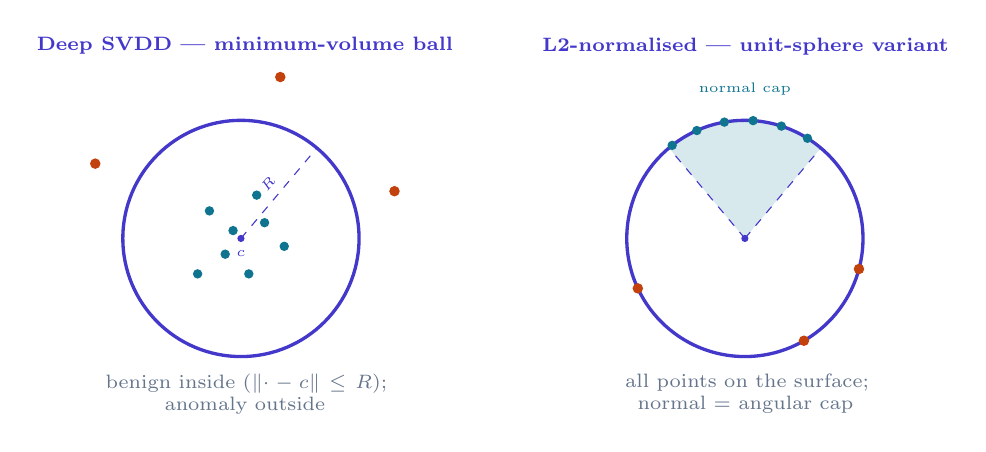
\begin{tikzpicture}

  \begin{scope}[local bounding box=PA]
    \draw[primary, very thick] (0,0) circle (1.5cm);
    \draw[primary, dashed] (0,0) -- (50:1.5)
         node[midway, above, sloped, font=\tiny\color{primary}] {$R$};
    \fill[primary] (0,0) circle (1.3pt) node[below=1pt, font=\tiny\color{primary}] {$c$};
    \foreach \p in {(0.3,0.2),(-0.4,0.35),(0.1,-0.45),(-0.2,-0.2),(0.55,-0.1),(-0.55,-0.45),(0.2,0.55),(-0.1,0.1)}
       {\fill[secondary] \p circle (1.7pt);}
    \foreach \p in {(1.95,0.6),(-1.85,0.95),(0.5,2.05)}
       {\fill[accent] \p circle (1.9pt);}
  \end{scope}
  \node[font=\bfseries\scriptsize\color{primary}, above=0.1cm of PA] {Deep SVDD --- minimum-volume ball};
  \node[font=\scriptsize\color{mute}, below=0.1cm of PA, text width=4cm, align=center]
       {benign inside ($\lVert\cdot - c\rVert \le R$); \\ anomaly outside};

  \begin{scope}[shift={(6.4,0)}, local bounding box=PB]
    \fill[secondary!16] (0,0) -- (50:1.5) arc (50:130:1.5) -- cycle;
    \draw[primary, very thick] (0,0) circle (1.5cm);
    \draw[primary, dashed] (0,0) -- (50:1.5);
    \draw[primary, dashed] (0,0) -- (130:1.5);
    \foreach \a in {58,72,86,100,114,128} {\fill[secondary] (\a:1.5) circle (1.7pt);}
    \foreach \a in {-15,205,300} {\fill[accent] (\a:1.5) circle (1.9pt);}
    \fill[primary] (0,0) circle (1.3pt);
    \node[font=\tiny\color{secondary}, above] at (90:1.7) {normal cap};
  \end{scope}
  \node[font=\bfseries\scriptsize\color{primary}, above=0.1cm of PB] {L2-normalised --- unit-sphere variant};
  \node[font=\scriptsize\color{mute}, below=0.1cm of PB, text width=4cm, align=center]
       {all points on the surface; \\ normal $=$ angular cap};

\end{tikzpicture}
\caption*{\small\textit{Figure 6 --- Two ways to realise ``inside $=$ in-class.'' Left: deep SVDD packs benign embeddings (teal) into a minimum-volume ball of radius $R$ around $c$; anomalies (amber) fall outside. Right: L2 normalisation places every point on the unit sphere's surface and ``normal'' becomes a learned angular cap. Both boundaries are learned from benign data.}}
\end{figure}

% =======================================================================
\section{Two operating modes --- default and strong}

The gateway runs in one of two configurations. The choice is an \textbf{operator-level setting} flipped by the admin, not a per-flow decision.

\begin{itemize}[leftmargin=*, itemsep=2pt]
  \item \textbf{Default mode --- low power, always on.} Smaller Mamba, smaller $K$ (e.g.\ $K=8$), \emph{only the anomaly head} active, no SHAP. Detection is on, the compute cost is small enough for continuous use, and both known and novel attacks are caught via the anomaly score alone.
  \item \textbf{Strong mode --- admin-switched, full pipeline.} Full Mamba, $K=32$, \emph{both} heads (anomaly via the projection MLP), plus SHAP on every alert. Switched on for an elevated threat level, an active investigation, a high-value time window, or simply maximum detection fidelity.
\end{itemize}

The same artifacts --- encoder $\theta_*$, classifier, projection, anomaly head --- serve both modes; what differs is which components are engaged and at what size. Both modes alert to the SOC; strong mode additionally produces per-packet SHAP attributions.

% ---- Figure 7: two-mode inference -------------------------------------
\begin{figure}[H]
\centering
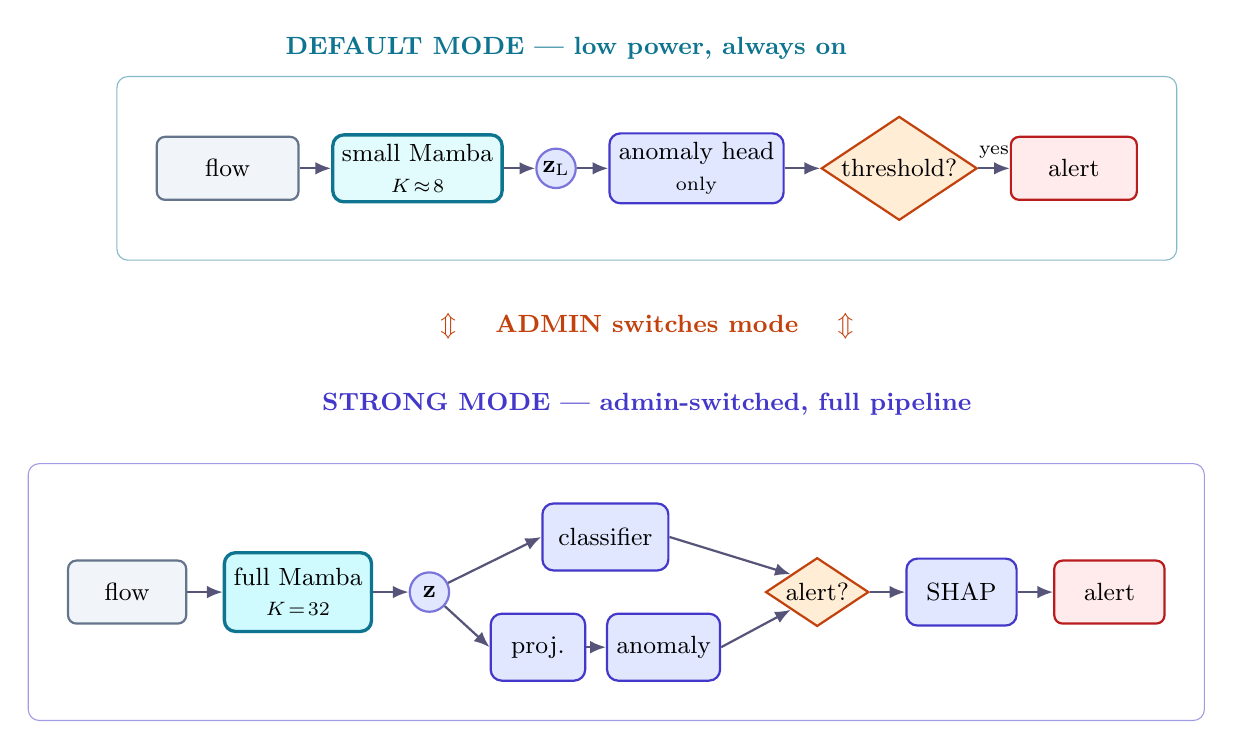
\begin{tikzpicture}[node distance=0.5cm and 0.55cm]

  \node[font=\bfseries\small\color{secondary}] (defhd) {DEFAULT MODE --- low power, always on};

  \node[data, below=0.85cm of defhd, xshift=-4.3cm, minimum width=1.8cm] (din) {flow};
  \node[brain, right=0.4cm of din, minimum width=2.0cm, minimum height=0.85cm, fill=secondarylight!60] (dmamba)
       {small Mamba \\ \scriptsize $K\!\approx\!8$};
  \node[bead, right=0.4cm of dmamba, minimum size=0.5cm, font=\small] (dz) {$\mathbf{z}_\text{L}$};
  \node[block, right=0.4cm of dz, minimum width=2.0cm] (dano) {anomaly head \\ \scriptsize only};
  \node[decision, right=0.45cm of dano] (dfuse) {threshold?};
  \node[signal, right=0.4cm of dfuse, minimum width=1.6cm] (dout) {alert};

  \draw[ar] (din) -- (dmamba);
  \draw[ar] (dmamba) -- (dz);
  \draw[ar] (dz) -- (dano);
  \draw[ar] (dano) -- (dfuse);
  \draw[ar] (dfuse) -- node[above, font=\scriptsize]{yes} (dout);

  \node[draw=secondary!50, rounded corners, fit=(din)(dout)(dmamba)(dano)(dfuse), inner sep=14pt] (sdef) {};

  \node[below=0.55cm of sdef, font=\bfseries\small\color{accent}] (sw)
       {$\Updownarrow$ \quad ADMIN switches mode \quad $\Updownarrow$};

  \node[font=\bfseries\small\color{primary}, below=0.45cm of sw] (strhd)
       {STRONG MODE --- admin-switched, full pipeline};

  \node[data, below=1.7cm of strhd, xshift=-6.6cm, minimum width=1.5cm] (sin) {flow};
  \node[brain, right=0.45cm of sin, minimum width=1.8cm, minimum height=1.0cm] (smamba)
       {full Mamba \\ \scriptsize $K\!=\!32$};
  \node[bead, right=0.45cm of smamba, minimum size=0.5cm, font=\small] (sz) {$\mathbf{z}$};
  \node[block, right=0.5cm of sz, yshift=-0.7cm, minimum width=1.2cm] (sproj)
       {proj.};
  \node[block, right=0.25cm of sproj, minimum width=1.4cm] (sano) {anomaly};
  \coordinate (smid) at ($(sproj.west)!0.5!(sano.east)$);
  \node[block, minimum width=1.6cm] (scls) at ([yshift=1.4cm]smid) {classifier};
  \node[decision, right=0.55cm of sano, yshift=0.7cm] (sfuse) {alert?};
  \node[block, right=0.45cm of sfuse, minimum width=1.4cm] (sshap) {SHAP};
  \node[signal, right=0.45cm of sshap, minimum width=1.4cm] (sout) {alert};

  \draw[ar] (sin) -- (smamba);
  \draw[ar] (smamba) -- (sz);
  \draw[ar] (sz) -- (scls.west);
  \draw[ar] (sz) -- (sproj.west);
  \draw[ar] (sproj) -- (sano);
  \draw[ar] (scls.east) -- (sfuse.north west);
  \draw[ar] (sano.east) -- (sfuse.south west);
  \draw[ar] (sfuse) -- (sshap);
  \draw[ar] (sshap) -- (sout);

  \node[draw=primary!50, rounded corners, fit=(sin)(sout)(scls)(sproj)(sano)(sfuse)(sshap), inner sep=14pt] (sstr) {};

\end{tikzpicture}
\caption*{\small\textit{Figure 7 --- The two operating modes. Default runs continuously on a small Mamba with only the anomaly head. Strong is switched on by the admin and engages the full pipeline: full Mamba, classifier, projected anomaly head, and SHAP. The admin chooses which mode is active; the gateway then runs entirely in that mode until the next switch.}}
\end{figure}

% =======================================================================
\section{Training --- three stages, then a loop}

The encoder is built first without labels, specialised with labels, then the anomaly head is fitted on top.

\subsection{Stage A --- pre-train the encoder, no labels}
Take a large set of \textbf{benign} flows. Randomly mask $\sim$15\% of packet positions in each sequence and train the Mamba encoder to predict the masked packets from context --- the SSL recipe pioneered by ET-BERT, applied to per-packet features. Output: an encoder $\theta_0$ that has learned what normal traffic looks like.

\subsection{Stage B --- fine-tune with labels}
Attach a fresh classification head on $\theta_0$ and jointly fine-tune the encoder and head on labelled CICIoT2023 attack data with focal loss. Output: the fine-tuned encoder $\theta_*$ and the trained classifier.

\subsection{Stage C --- fit the anomaly head}
Freeze $\theta_*$. Push a held-out benign set through it to get embeddings, train the projection MLP, and fit deep SVDD on the projected embeddings. Calibrate the threshold at the 99th percentile of benign scores.

\subsection{The loop --- absorbing new attack types}
When an unseen attack appears, the system does \emph{not} need full retraining:
\begin{enumerate}[leftmargin=*, itemsep=2pt]
  \item The anomaly head flags the novel attack on day zero --- it just looks unlike normal.
  \item The SOC labels a sample of the flagged flows as a new class.
  \item Extend the classifier softmax by one class and fine-tune \textbf{only the classifier head}, with a small replay buffer of old classes to prevent forgetting. The encoder stays frozen. Minutes, not days.
  \item Optionally recalibrate the anomaly threshold on a fresh benign set.
\end{enumerate}
Full encoder retraining is triggered only if the benign distribution itself shifts (new device types added). ``What's normal'' lives in the expensive encoder; ``what's malicious'' lives in the cheap heads.

% ---- Figure 8: training stages ----------------------------------------
\begin{figure}[H]
\centering
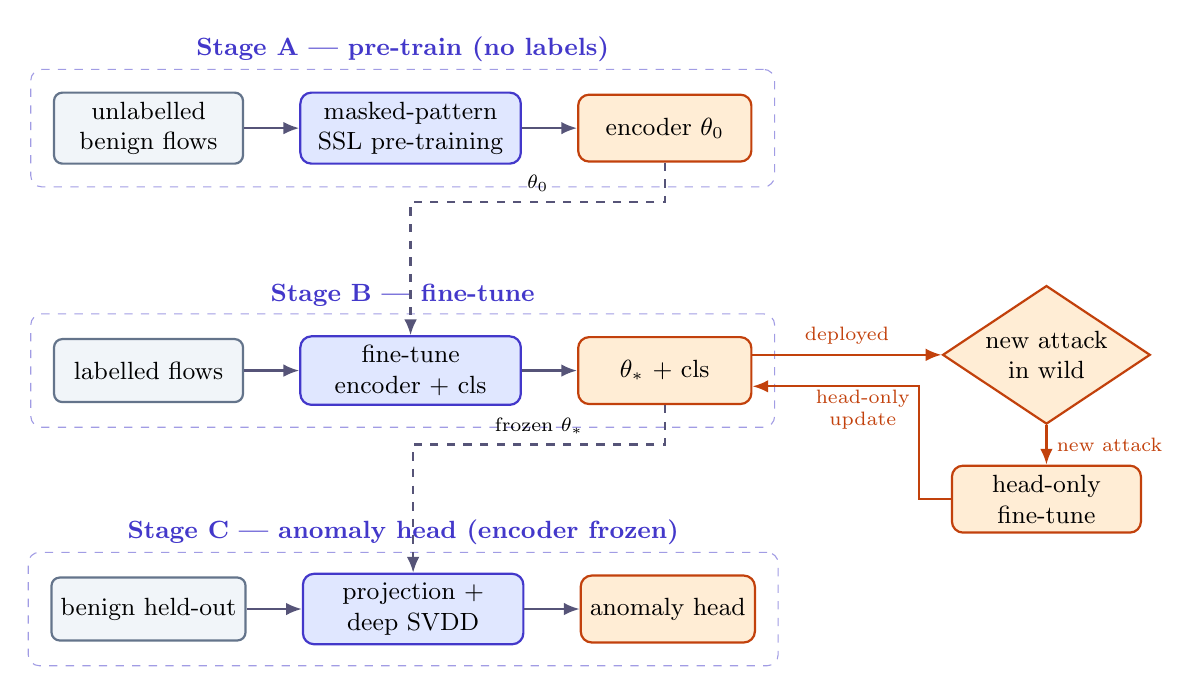
\begin{tikzpicture}[node distance=0.55cm and 0.7cm]

  \node[data, minimum width=2.4cm] (a1) {unlabelled \\ benign flows};
  \node[block, right=of a1, minimum width=2.8cm] (a2)
       {masked-pattern \\ SSL pre-training};
  \node[art, right=of a2, minimum width=2.2cm] (a3) {encoder $\theta_0$};
  \node[draw=primary!50, dashed, rounded corners, fit=(a1)(a3), inner sep=8pt,
        label={[font=\small\bfseries\color{primary}, above=-1pt]:Stage A --- pre-train (no labels)}] (sA) {};
  \draw[ar] (a1) -- (a2);
  \draw[ar] (a2) -- (a3);

  \node[data, minimum width=2.4cm, below=2.2cm of a1] (b1) {labelled flows};
  \node[block, right=of b1, minimum width=2.8cm] (b2)
       {fine-tune \\ encoder + cls};
  \node[art, right=of b2, minimum width=2.2cm] (b3) {$\theta_*$ + cls};
  \node[draw=primary!50, dashed, rounded corners, fit=(b1)(b3), inner sep=8pt,
        label={[font=\small\bfseries\color{primary}, above=-1pt]:Stage B --- fine-tune}] (sB) {};
  \draw[ar] (b1) -- (b2);
  \draw[ar] (b2) -- (b3);
  \draw[dar] (a3.south) -- ++(0,-0.5) -| node[pos=0.25, above, font=\scriptsize]{$\theta_0$} (b2.north);

  \node[data, minimum width=2.4cm, below=2.2cm of b1] (c1) {benign held-out};
  \node[block, right=of c1, minimum width=2.8cm] (c2)
       {projection + \\ deep SVDD};
  \node[art, right=of c2, minimum width=2.2cm] (c3) {anomaly head};
  \node[draw=primary!50, dashed, rounded corners, fit=(c1)(c3), inner sep=8pt,
        label={[font=\small\bfseries\color{primary}, above=-1pt]:Stage C --- anomaly head (encoder frozen)}] (sC) {};
  \draw[ar] (c1) -- (c2);
  \draw[ar] (c2) -- (c3);
  \draw[dar] (b3.south) -- ++(0,-0.5) -| node[pos=0.25, above, font=\scriptsize]{frozen $\theta_*$} (c2.north);

  \node[decision, right=2.4cm of b3, yshift=0.2cm, fill=accentlight] (newatk)
       {new attack \\ in wild};
  \node[block, below=0.5cm of newatk, minimum width=2.4cm, fill=accentlight, draw=accent] (heads)
       {head-only \\ fine-tune};

  \draw[ar, draw=accent, line width=0.8pt] ([yshift=0.2cm]b3.east) -- node[above, font=\scriptsize\color{accent}]{deployed} (newatk.west);
  \draw[ar, draw=accent, line width=0.8pt] (newatk) -- node[right, font=\scriptsize\color{accent}]{new attack} (heads);
  \draw[ar, draw=accent, line width=0.8pt]
    (heads.west) -- ++(-0.4, 0)
    |- ([yshift=-0.2cm]b3.east);

  \node[font=\scriptsize\color{accent}, align=center]
    at ([xshift=1.4cm, yshift=-0.5cm]b3.east)
    {head-only \\ update};

\end{tikzpicture}
\caption*{\small\textit{Figure 8 --- The three training stages produce the deployed detector. The amber loop on the right is the progressive-learning path: a new attack triggers a head-only re-train --- the expensive encoder stays put.}}
\end{figure}

\subsection{Continual learning --- the correlation problem}
The hard case is correlation: a new attack class often resembles an existing one (a new DDoS variant looks like the standard DDoS class), so naive head retraining quietly confuses them. Three failure modes appear --- \textbf{catastrophic forgetting} (the head drifts toward the new class), \textbf{probability-mass theft} (the new softmax dimension steals confidence from the correlated class), and \textbf{spurious hard labels} (boundary flows forced into one class, hiding the ambiguity from the analyst). Before adding a class, embed the candidate flows through the frozen encoder and inspect where they land.

% ---- Figure 9: embedding scenarios ------------------------------------
\begin{figure}[H]
\centering
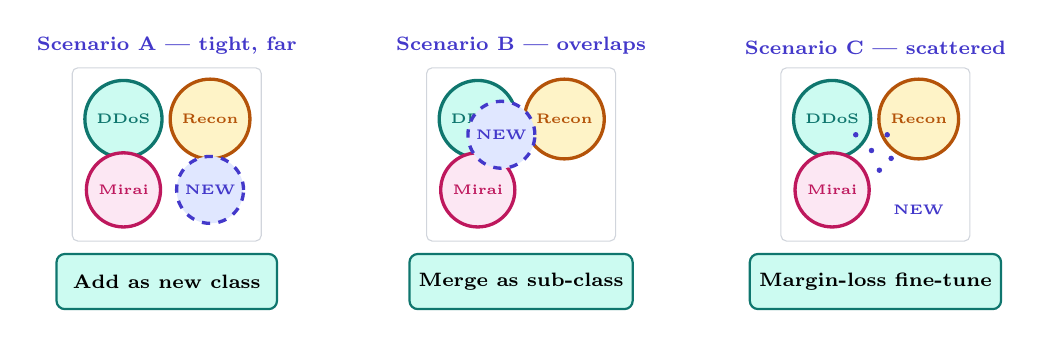
\begin{tikzpicture}[
    clusterN/.style={circle, draw=clsN, dashed, very thick, fill=clsNlight, inner sep=0pt, minimum size=0.85cm, font=\tiny\color{clsN}\bfseries},
    dotN/.style={circle, fill=clsN, inner sep=0.7pt},
    scene/.style={draw=mute!30, rounded corners=2pt},
  ]

  \begin{scope}[local bounding box=A]
    \draw[scene] (-1.2,-1.1) rectangle (1.2,1.1);
    \node[circle, draw=clsA, very thick, fill=clsAlight, minimum size=0.85cm, font=\tiny\color{clsA}\bfseries] at (-0.55, 0.45) {DDoS};
    \node[circle, draw=clsB, very thick, fill=clsBlight, minimum size=0.85cm, font=\tiny\color{clsB}\bfseries] at ( 0.55, 0.45) {Recon};
    \node[circle, draw=clsC, very thick, fill=clsClight, minimum size=0.85cm, font=\tiny\color{clsC}\bfseries] at (-0.55, -0.45) {Mirai};
    \node[clusterN] at (0.55, -0.45) {NEW};
  \end{scope}
  \node[font=\bfseries\scriptsize\color{primary}, above=0.05cm of A] {Scenario A --- tight, far};
  \node[result, below=0.15cm of A, minimum width=2.8cm, fill=clsAlight, draw=clsA, font=\scriptsize, minimum height=0.7cm]
       {\textbf{Add as new class}};

  \begin{scope}[local bounding box=B, shift={(4.5,0)}]
    \draw[scene] (-1.2,-1.1) rectangle (1.2,1.1);
    \node[circle, draw=clsA, very thick, fill=clsAlight, minimum size=0.85cm, font=\tiny\color{clsA}\bfseries] at (-0.55, 0.45) {DDoS};
    \node[circle, draw=clsB, very thick, fill=clsBlight, minimum size=0.85cm, font=\tiny\color{clsB}\bfseries] at ( 0.55, 0.45) {Recon};
    \node[circle, draw=clsC, very thick, fill=clsClight, minimum size=0.85cm, font=\tiny\color{clsC}\bfseries] at (-0.55, -0.45) {Mirai};
    \node[clusterN] at (-0.25, 0.25) {NEW};
  \end{scope}
  \node[font=\bfseries\scriptsize\color{primary}, above=0.05cm of B] {Scenario B --- overlaps};
  \node[result, below=0.15cm of B, minimum width=2.8cm, fill=clsAlight, draw=clsA, font=\scriptsize, minimum height=0.7cm]
       {\textbf{Merge as sub-class}};

  \begin{scope}[local bounding box=C, shift={(9.0,0)}]
    \draw[scene] (-1.2,-1.1) rectangle (1.2,1.1);
    \node[circle, draw=clsA, very thick, fill=clsAlight, minimum size=0.85cm, font=\tiny\color{clsA}\bfseries] at (-0.55, 0.45) {DDoS};
    \node[circle, draw=clsB, very thick, fill=clsBlight, minimum size=0.85cm, font=\tiny\color{clsB}\bfseries] at ( 0.55, 0.45) {Recon};
    \node[circle, draw=clsC, very thick, fill=clsClight, minimum size=0.85cm, font=\tiny\color{clsC}\bfseries] at (-0.55, -0.45) {Mirai};
    \node[dotN] at (-0.05, 0.05) {};
    \node[dotN] at ( 0.15, 0.25) {};
    \node[dotN] at (-0.25, 0.25) {};
    \node[dotN] at ( 0.2, -0.05) {};
    \node[dotN] at ( 0.05, -0.2) {};
    \node[font=\tiny\color{clsN}\bfseries] at (0.55, -0.7) {NEW};
  \end{scope}
  \node[font=\bfseries\scriptsize\color{primary}, above=0.05cm of C] {Scenario C --- scattered};
  \node[result, below=0.15cm of C, minimum width=2.8cm, fill=clsAlight, draw=clsA, font=\scriptsize, minimum height=0.7cm]
       {\textbf{Margin-loss fine-tune}};

\end{tikzpicture}
\caption*{\small\textit{Figure 9 --- Three embedding-space scenarios for a new attack class (existing classes solid, new class dashed indigo). The geometry dictates strategy: tight \& far $\to$ add; overlapping $\to$ merge as sub-class; scattered between $\to$ enforce separation via margin loss. Run before any softmax change is committed.}}
\end{figure}

\subsection{The update protocol --- four defences, in order}
\begin{enumerate}[leftmargin=*, itemsep=2pt]
  \item \textbf{Replay buffer (primary).} Persist $\sim$100--500 labelled flows per existing class; batch them in on every fine-tuning step so the head still sees every old class. Cheap, well-studied, usually enough.
  \item \textbf{Knowledge distillation (Learning-without-Forgetting).} Regularise the new head toward agreeing with the old head on old-class data --- one extra forward pass through the frozen old head.
  \item \textbf{Embedding-space sanity check.} Locate the new samples relative to existing class prototypes; branch on the three scenarios above.
  \item \textbf{Surface uncertainty, don't force labels.} If the softmax is split (55\% NEW, 40\% DDoS), pass both confidences plus the anomaly score and SHAP to the SOC instead of forcing a hard label.
\end{enumerate}

% ---- Figure 10: update protocol ---------------------------------------
\begin{figure}[H]
\centering
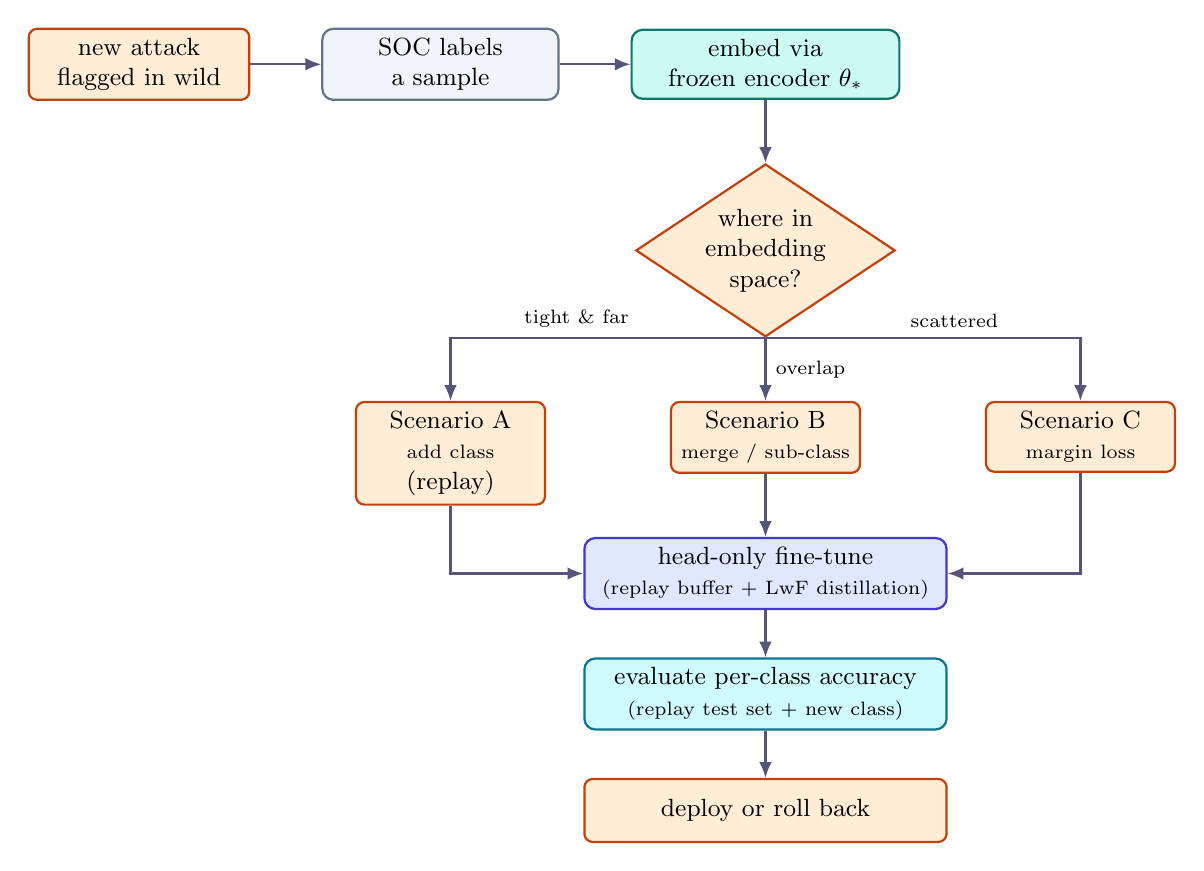
\begin{tikzpicture}[node distance=0.6cm and 0.9cm]

  \node[data, fill=accentlight, draw=accent, minimum width=2.8cm] (in) {new attack \\ flagged in wild};
  \node[block, right=of in, minimum width=3.0cm, fill=mutelight, draw=mute] (label)
       {SOC labels \\ a sample};
  \node[block, right=of label, minimum width=3.4cm, fill=precfplight, draw=precfp] (embed)
       {embed via \\ frozen encoder $\theta_*$};

  \draw[ar] (in) -- (label);
  \draw[ar] (label) -- (embed);

  \node[decision, below=0.8cm of embed, fill=accentlight, draw=accent] (where)
       {where in \\ embedding \\ space?};
  \draw[ar] (embed) -- (where);

  \node[result, below=0.8cm of where, xshift=-4.0cm] (sA)
       {Scenario A \\ \scriptsize add class \\ (replay)};
  \node[result, below=0.8cm of where] (sB)
       {Scenario B \\ \scriptsize merge / sub-class};
  \node[result, below=0.8cm of where, xshift=4.0cm] (sC)
       {Scenario C \\ \scriptsize margin loss};

  \draw[ar] (where.south) -| node[pos=0.3, above, font=\scriptsize] {tight \& far} (sA.north);
  \draw[ar] (where) -- node[right, font=\scriptsize] {overlap} (sB);
  \draw[ar] (where.south) -| node[pos=0.3, above, font=\scriptsize] {scattered} (sC.north);

  \node[block, below=0.8cm of sB, minimum width=4.6cm, fill=primarylight, draw=primary] (update)
       {head-only fine-tune \\ \scriptsize (replay buffer + LwF distillation)};

  \draw[ar] (sA.south) |- (update.west);
  \draw[ar] (sB) -- (update);
  \draw[ar] (sC.south) |- (update.east);

  \node[block, below=of update, minimum width=4.6cm, fill=secondarylight, draw=secondary] (eval)
       {evaluate per-class accuracy \\ \scriptsize (replay test set + new class)};
  \draw[ar] (update) -- (eval);

  \node[result, below=of eval, minimum width=4.6cm] (out)
       {deploy or roll back};
  \draw[ar] (eval) -- (out);

\end{tikzpicture}
\caption*{\small\textit{Figure 10 --- The progressive-learning update protocol. The encoder is never touched. The embedding-space scenario decides add / merge / separate; the head is fine-tuned with replay and distillation; per-class accuracy is checked before deploying. If any existing class regresses beyond a set threshold, the update is rolled back automatically.}}
\end{figure}

% =======================================================================
\section{Deployment and quantisation}

The deployed detector must fit on gateway-class hardware. Quantisation --- storing weights and activations in fewer bits than fp32 --- is the standard route to a smaller, faster model. The question is whether Mamba quantises cleanly, since most published quantisation work targets transformers.

\begin{tcolorbox}[idea]
Mamba does quantise, but the selective state-space core has activation outliers that compound through its recurrence. The practical strategy is \emph{mixed precision}: int8 for the linear projections (most of the parameters), fp16 for the SSM core (the sensitive part).
\end{tcolorbox}

A Mamba block has two parts. The \textbf{linear projections} (input, gating, output) dominate the parameter count and quantise cleanly to int8. The \textbf{selective state-space core} ($\Delta$, the input-dependent $B$, $C$, and the recurrent scan) has activation outliers and compounds error along the sequence; int8 cannot represent these without large error. Headline recipe: int8 the projections, fp16 the SSM core --- size savings come mostly from the projections anyway.

% ---- Figure 11: precision split ---------------------------------------
\begin{figure}[H]
\centering
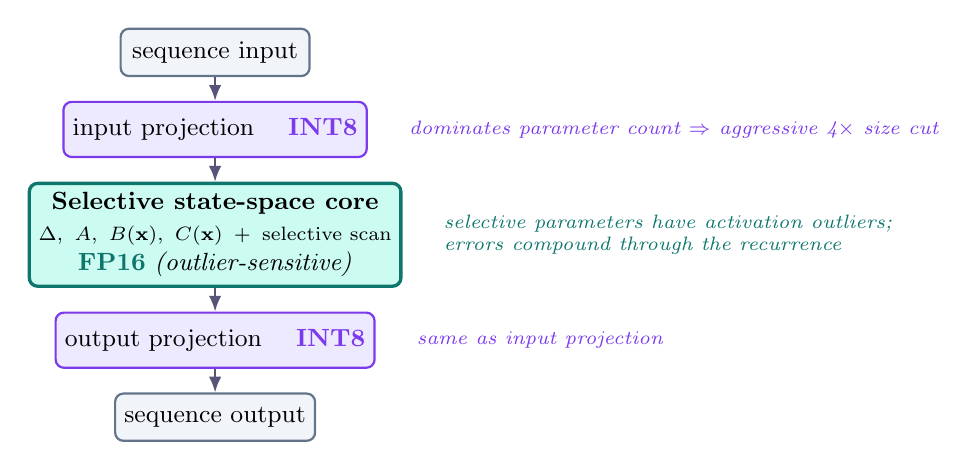
\begin{tikzpicture}[node distance=0.3cm and 0.6cm]

  \node[data, minimum width=2.4cm, minimum height=0.6cm] (in) {sequence input};
  \node[int8, below=of in] (proj1) {input projection \quad\textcolor{precint}{\textbf{INT8}}};
  \node[fp16, below=of proj1] (ssm)
       {\textbf{Selective state-space core} \\
        \scriptsize $\Delta,~A,~B(\mathbf{x}),~C(\mathbf{x})$ \,+\, selective scan \\
        \textcolor{precfp}{\textbf{FP16}} \emph{(outlier-sensitive)}};
  \node[int8, below=of ssm] (proj2) {output projection \quad\textcolor{precint}{\textbf{INT8}}};
  \node[data, below=of proj2, minimum width=2.4cm, minimum height=0.6cm] (out) {sequence output};

  \draw[ar] (in) -- (proj1);
  \draw[ar] (proj1) -- (ssm);
  \draw[ar] (ssm) -- (proj2);
  \draw[ar] (proj2) -- (out);

  \node[font=\scriptsize\itshape\color{precint}, align=left, right=0.4cm of proj1]
       {dominates parameter count $\Rightarrow$ aggressive 4$\times$ size cut};
  \node[font=\scriptsize\itshape\color{precfp}, align=left, right=0.4cm of ssm]
       {selective parameters have activation outliers;\\errors compound through the recurrence};
  \node[font=\scriptsize\itshape\color{precint}, align=left, right=0.4cm of proj2]
       {same as input projection};

\end{tikzpicture}
\caption*{\small\textit{Figure 11 --- Mixed-precision split inside a Mamba block. Linear projections (violet, int8) carry most of the weights and quantise cleanly; the selective SSM core (teal, fp16) is sensitive and stays at higher precision. This is the practical compromise across the 2024--25 Mamba quantisation literature (Q-Mamba, MambaQuant, PTQ4SSM).}}
\end{figure}

The deployed model is reported in three precisions so the operator can choose:

\begin{center}
\small
\begin{tabularx}{\linewidth}{@{}Xccc@{}}
\toprule
\textbf{Configuration} & \textbf{Size} & \textbf{p95 latency} & \textbf{Accuracy hit} \\
\midrule
fp32 (baseline)                                 & $1.0\times$          & $1.0\times$        & --- \\
int8 PTQ everywhere                             & $0.25\times$         & ${\sim}0.5\times$  & risk on SSM core \\
\textbf{Mixed precision (recommended)}          & $\approx 0.30\times$ & ${\sim}0.55\times$ & smallest drop \\
\bottomrule
\end{tabularx}
\end{center}

If int8-everywhere degrades accuracy too far, mixed precision is the recommended configuration. Quantisation-aware training is the fallback for the SSM core if even fp16 leaves quality on the table.

% =======================================================================
\section{Evaluation}

\subsection{Datasets}
\textbf{CICIoT2023} (primary). \textbf{TON\_IoT} for cross-dataset generalisation --- the trained model evaluated on a dataset it has never seen. \textbf{IoT-23} for a real-world malware check (Mirai, Torii, Okiru, Gafgyt).

\subsection{Baselines --- and what each one is for}
\begin{itemize}[leftmargin=*, itemsep=2pt]
  \item \textbf{ET-BERT} --- the published-SOTA upper bound. Quantifies the accuracy given up by going to Mamba.
  \item \textbf{CNN-BiLSTM on aggregated statistics} --- the representation control. Isolates the gain from the flow-pattern input.
  \item \textbf{XGBoost on aggregated statistics} --- the classical-floor challenge. Gradient-boosted trees on hand-crafted features are routinely competitive in IDS literature. The deep detector earns its complexity only if it beats XGBoost on what XGBoost cannot target: \textbf{zero-day detection} (XGBoost is supervised-only), \textbf{cross-dataset transfer}, and \textbf{adversarial robustness}. If XGBoost matches in-distribution, that is reported as a finding.
  \item \textbf{Isolation Forest} --- the classical unsupervised floor for the anomaly head.
\end{itemize}

\subsection{Metrics}
Per-class precision / recall / F1. PR-AUC (the honest metric under heavy class imbalance). Inference latency p50 / p95 / p99 per flow. Model size in MB after int8 quantisation.

\subsection{Adversarial study}
Fast Gradient Sign Method (FGSM) on the per-packet sequence, perturbations clipped to valid feature ranges. Detection rate vs.\ perturbation magnitude $\varepsilon$, plotted for both heads. Secondary check: SHAP attribution patterns on adversarial inputs tend to differ from clean inputs --- a useful fallback signal.

\subsection{Zero-day proxy}
Leave-one-class-out: hide an attack class from the supervised head during Stage B, then measure how well the anomaly head detects it at test time. Repeat per class. This is the concrete answer to ``how do you evaluate something you haven't trained on.''

% =======================================================================
\section{Plan, deliverables, risks}

\subsection{Twelve-week plan}
Weeks 1--2 setup and dataset validation; week 3 flow-pattern extractor, preprocessing transforms, and classical baselines; weeks 4--5 Stage A pre-training; week 6 Stage B fine-tuning and CNN-BiLSTM + ET-BERT comparison; week 7 Stage C anomaly head and leave-one-class-out; week 8 TON\_IoT + IoT-23 evaluation; week 9 SHAP integration and t-SNE/UMAP embedding analysis; week 10 FGSM adversarial study; week 11 int8 quantisation and gateway latency benchmark; week 12 stretch goal, final report, presentation.

\subsection{Deliverables}
A reproducible code repository covering the full pipeline. The pre-trained Mamba encoder checkpoint $\theta_*$ released with the report. A benchmark table covering Mamba vs.\ ET-BERT vs.\ CNN-BiLSTM vs.\ XGBoost vs.\ Isolation Forest across CICIoT2023, TON\_IoT, IoT-23. FGSM degradation curves. Latency / memory profile on gateway hardware. Written report.

\subsection{Risks --- and what I do about them}
\begin{tcolorbox}[warnbox]
\begin{itemize}[leftmargin=*, itemsep=1pt, topsep=0pt]
  \item \textbf{Pre-training compute blows budget.} Warm-start from a public Mamba checkpoint and adapt on benign IoT traffic rather than train from scratch.
  \item \textbf{Class imbalance hides minority-class failure.} Focal loss + always report per-class metrics.
  \item \textbf{Cross-dataset accuracy drop.} Measure honestly; this is the standard caveat in IDS literature, not a failure mode to hide.
  \item \textbf{Edge memory overrun.} Int8 quantise, fall back to a smaller Mamba, reduce $K$ as a last resort.
  \item \textbf{Adversarial sensitivity.} The FGSM study quantifies it; the SHAP fingerprint is a secondary defence.
\end{itemize}
\end{tcolorbox}

\subsection{Stretch goals}
\begin{itemize}[leftmargin=*, itemsep=1pt]
  \item Swap Mamba $\to$ Mamba-2 (Structured State Space Duality) if latency headroom allows.
  \item Add an E-GraphSAGE branch over a per-window device-communication graph.
  \item Federated pre-training across multiple homes / sites.
\end{itemize}

% =======================================================================
\section*{Key references}
\footnotesize
\begin{itemize}[leftmargin=*, itemsep=1pt]
  \item \textbf{NetMamba}, Wang et al.\ 2024 --- \href{https://arxiv.org/abs/2405.11449}{arxiv.org/abs/2405.11449}
  \item \textbf{ET-BERT}, Lin et al.\ WWW 2022 --- \href{https://arxiv.org/abs/2202.06335}{arxiv.org/abs/2202.06335}
  \item \textbf{Mamba}, Gu \& Dao 2023 --- \href{https://arxiv.org/abs/2312.00752}{arxiv.org/abs/2312.00752}
  \item \textbf{Mamba-2 / SSD}, Dao \& Gu 2024 --- \href{https://arxiv.org/abs/2405.21060}{arxiv.org/abs/2405.21060}
  \item \textbf{CICIoT2023}, Neto et al.\ 2023 --- \href{https://www.mdpi.com/1424-8220/23/13/5941}{mdpi.com/1424-8220/23/13/5941}
  \item \textbf{Deep SVDD}, Ruff et al.\ ICML 2018 --- the one-class anomaly scorer.
  \item \textbf{SHAP}, Lundberg \& Lee, NeurIPS 2017 --- attributions that double as feature importance.
  \item \textbf{t-SNE}, van der Maaten \& Hinton, JMLR 2008; \textbf{UMAP}, McInnes et al.\ 2018 --- \href{https://arxiv.org/abs/1802.03426}{arxiv.org/abs/1802.03426}
  \item \textbf{E-GraphSAGE}, Lo et al. --- \href{https://arxiv.org/abs/2103.16329}{arxiv.org/abs/2103.16329}
\end{itemize}

\end{document}
